\documentclass[14pt,a4paper]{extarticle}
\usepackage{../templates/preamble}

\newcommand{\reportof}{практической работе №6}
\newcommand{\theme}{Частные производные функций нескольких переменных}

\begin{document}
\begin{titlepage}
    \begin{center}
        {\bfseries
        МИНОБРНАУКИ РОССИИ\par
        САНКТ-ПЕТЕРБУРГСКИЙ ГОСУДАРСТВЕННЫЙ\par
        ЭЛЕКТРОТЕХНИЧЕСКИЙ УНИВЕРСИТЕТ\par
        <<ЛЭТИ>> ИМ. В.И. УЛЬЯНОВА (ЛЕНИНА)\par
        Кафедра \department

        \vspace{0.23\textheight}
        ОТЧЁТ\par
        по \reportof\par
        по дисциплине <<\discipline>>\par
        Тема: \theme
        \vspace{0.28\textheight}
        }
        \begin{table}[!ht]
            \begin{tabularx}{\textwidth}{p{60mm}X>{\centering\arraybackslash}p{45mm}}
                Студент гр. 4352 & \_\_\_\_\_\_\_\_\_\_\_\_\_\_\_\_\_\_\_\_ & {Даричев Е. М.} \\ [5.4mm]  % Line height
                Преподаватель    & \_\_\_\_\_\_\_\_\_\_\_\_\_\_\_\_\_\_\_\_ & {\teacher} \\ [5.4mm]
            \end{tabularx}
        \end{table}

        Санкт-Петербург\par
        \yyear
    \end{center}
\end{titlepage}
\setcounter{page}{2}

\section*{Цель работы}
        Изучить методы работы с частными производными
функций нескольких переменных и научиться вычислять 
MSE функций нескольких переменных.


\section*{Отчёт о проделанной работе}
Чтобы вычислить среднее квадратичное для функций нужно взять каждую пару значений $(x_1,x_2)$
из списка объектов и подставить их в функцию с помощью subs. Затем для каждого объекта вычисляется
разность между предсказанным значением и целевым значением, эта разность возводится в квадрат.
Все квадраты ошибок складываются и делятся на их количество (рис. \ref{pic:cod}).

\begin{figure}[ht!]
    \centering
    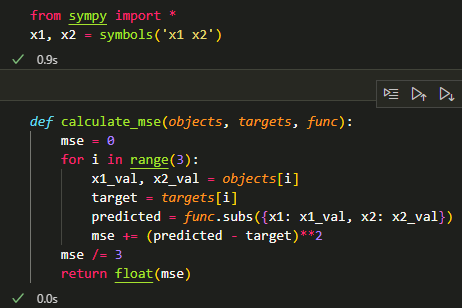
\includegraphics[width=0.7\linewidth]{figures/1.png}
    \caption{Код для нахождения MSE}
    \label{pic:cod}
\end{figure}

В первом наборе данных функция
$f_1=-2x_2+x_1-7$ имеет значение MSE, чем функция $f_2=20x_2+3x_1-4$ (рис. \ref{pic:mse1}).

\begin{figure}[ht!]
    \centering
    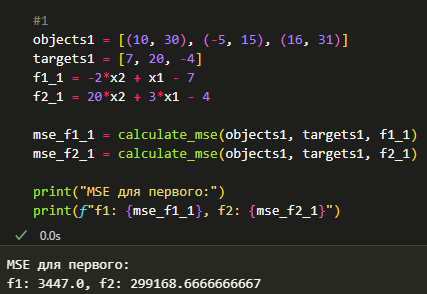
\includegraphics[width=0.9\linewidth]{figures/1.1.png}
    \caption{MSE для первого набора}
    \label{pic:mse1}
\end{figure}

В первом наборе данных функция
$f_1=-2x_2-x_1+60$ имеет значение MSE, чем функция $f_2=2x_2+17x_1-9$ (рис. \ref{pic:mse2}).

\begin{figure}[ht!]
    \centering
    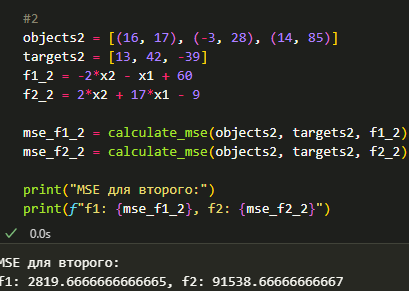
\includegraphics[width=0.9\linewidth]{figures/1.2.png}
    \caption{MSE для второго набора}
    \label{pic:mse2}
\end{figure}

В первом наборе данных функция
$f_1=-4x_2+7x_1-11$ имеет значение MSE, чем функция $f_2=-0.5x_2+9x_1-400$ (рис. \ref{pic:mse3}).

\begin{figure}[ht!]
    \centering
    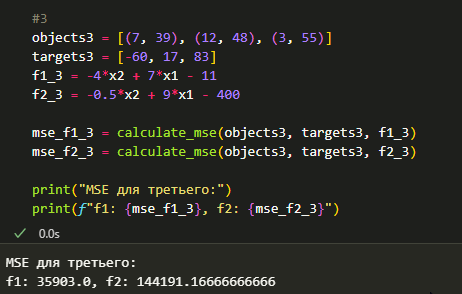
\includegraphics[width=0.9\linewidth]{figures/1.3.png}
    \caption{MSE для третьего набора}
    \label{pic:mse3}
\end{figure}

Нахождение частные производных:


\begin{enumerate}
    \item 
    \[
    f(x_1, x_2) = 10x_1 - 5x_2
    \]
    \[
    \frac{\partial f}{\partial x_1} = 10 - 0 = 10
    \]
    \[
    \frac{\partial f}{\partial x_2} = 0 - 5 = -5
    \]

    \item 
    \[
    f(x_1, x_2) = 3x_1 + 4x_2 + 7
    \]
    \[
    \frac{\partial f}{\partial x_1} = 3 + 0 + 0 = 3
    \]
    \[
    \frac{\partial f}{\partial x_2} = 0 + 4 + 0 = 4
    \]

    \item 
    \[
    f(x_1, x_2) = x_1^2
    \]
    \[
    \frac{\partial f}{\partial x_1} = 2x_1
    \]
    \[
    \frac{\partial f}{\partial x_2} = 0
    \]

    \item 
    \[
    f(x_1, x_2, x_3) = x_1 + 5x_2 - 6x_3 + 3
    \]
    \[
    \frac{\partial f}{\partial x_1} = 1 + 0 + 0 + 0 = 1
    \]
    \[
    \frac{\partial f}{\partial x_2} = 0 + 5 + 0 + 0 = 5
    \]
    \[
    \frac{\partial f}{\partial x_3} = 0 - 6 + 0 + 0 = -6
    \]

    \item 
    \[
    f(x_1, x_2, x_3) = 10x_1 - x_1^2 + 4x_1^3
    \]
    \[
    \frac{\partial f}{\partial x_1} = 10 - 2x_1 + 12x_1^2
    \]
    \[
    \frac{\partial f}{\partial x_2} = 0
    \]
    \[
    \frac{\partial f}{\partial x_3} = 0
    \]

    \item 
    \[
    f(x_1, x_2, x_3) = x_1^2 + 12x_1x_2 + 4x_2^3 + x_3
    \]
    \[
    \frac{\partial f}{\partial x_1} = 2x_1 + 12x_2
    \]
    \[
    \frac{\partial f}{\partial x_2} = 12x_1 + 12x_2^2
    \]
    \[
    \frac{\partial f}{\partial x_3} = 1
    \]
\end{enumerate}

Частные производные среднеквадратичной ошибки можно найти с помощью sympy (рис. \ref{pic:mse}).

\begin{figure}[ht!]
    \centering
    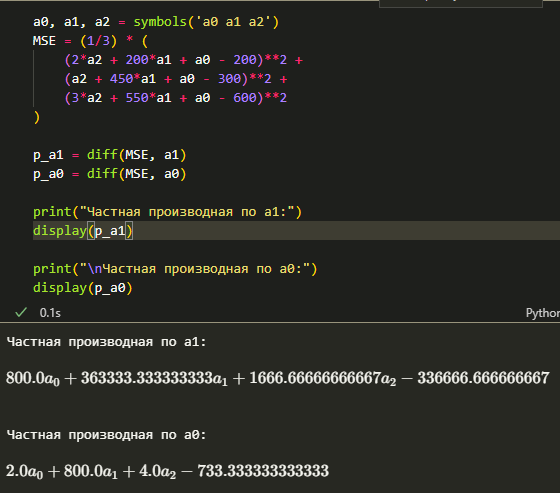
\includegraphics[width=0.9\linewidth]{figures/3.png}
    \caption{Производные MSE по $a_0$ и $a_1$}
    \label{pic:mse}
\end{figure}

Функция среднеквадратичной ошибки для четвёртого задания задаётся как:
\[
\mathtt{MSE} = \frac{1}{3} \sum_{i=1}^3 \left( \mathtt{Area}_i - (a_0 + a_1 \cdot \mathtt{Price}_i + a_2 \cdot \mathtt{Floors}_i) \right)^2,
\]
Частные производные MSE по коэффициентам $a_0$, $a_1$ и $a_2$:
\[
\frac{\partial \mathtt{MSE}}{\partial a_0} = -\frac{2}{3} \sum_{i=1}^3 \left( \mathtt{Area}_i - (a_0 + a_1 \cdot \mathtt{Price}_i + a_2 \cdot \mathtt{Floors}_i) \right),
\]
\[
\frac{\partial \mathtt{MSE}}{\partial a_1} = -\frac{2}{3} \sum_{i=1}^3 \left( \mathtt{Area}_i - (a_0 + a_1 \cdot \mathtt{Price}_i + a_2 \cdot \mathtt{Floors}_i) \right) \cdot \mathtt{Price}_i,
\]
\[
\frac{\partial \mathtt{MSE}}{\partial a_2} = -\frac{2}{3} \sum_{i=1}^3 \left( \mathtt{Area}_i - (a_0 + a_1 \cdot \mathtt{Price}_i + a_2 \cdot \mathtt{Floors}_i) \right) \cdot \mathtt{Floors}_i.
\]

Далее с помощью библиотеки sympy можно найти все необходимые
производные и предсказать площадь дома,
в этом случае точкой минимума являются найденные коэффициенты (рис. \ref{pic:house}).

\begin{figure}[ht!]
    \centering
    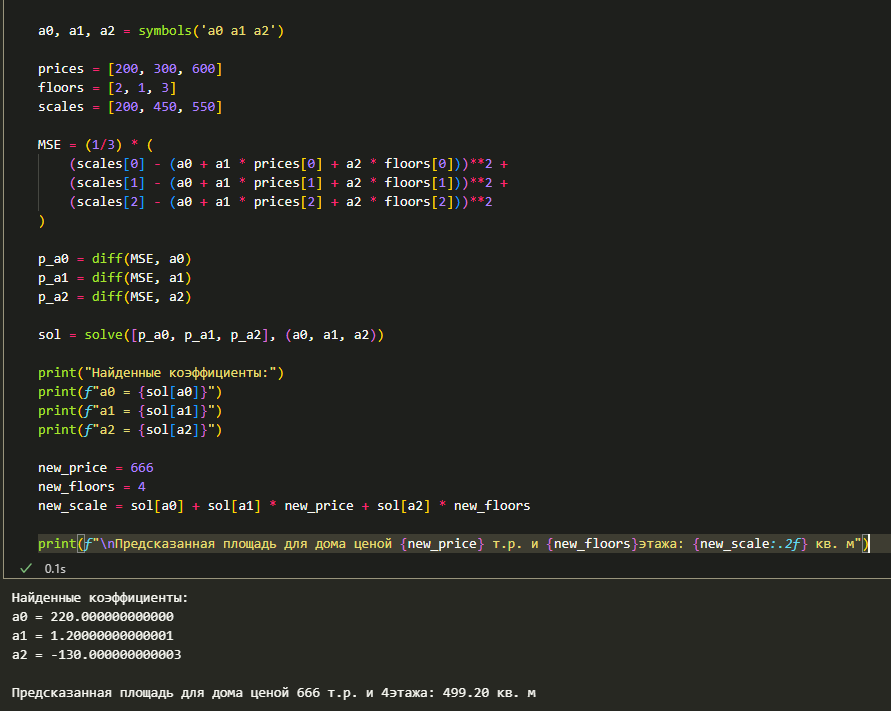
\includegraphics[width=0.7\linewidth]{figures/4.png}
    \caption{Предсказание цены дома}
    \label{pic:house}
\end{figure}

Полученная функция для площади имеет вид, MSE равно 0:
\begin{equation}
    - 130.0 \mathtt{floor} + 1.2 \mathtt{price} + 220.0
\end{equation}

\section*{Вывод.}

В ходе работы были изучены частные производные функции нескольких переменных,
а также метод нахождения среднеквадратичной ошибки для таких функций.

\end{document}